\chapter{簡介}
\label{ch:introduction}

\section{研究動機}
\label{sec:motivation}

羽球國際賽事的完整轉播影片大量公開於網路，記錄了選手每回合攻防的過程。教練與選手想從中歸納對手的慣用球路，研究者想統計戰術或訓練預測模型，真正需要的都不是影片本身，而是逐拍的資料，像是每回合有幾拍、每拍是什麼球種等等。影片並不直接提供這些資訊，目前仍須由人標記。ShuttleSet~\cite{shuttleset} 等羽球資料集即以人工標記建立，自動定位擊球影格的研究~\cite{chien2023hitframe} 也以減少這類人工作業為出發點。

在嘗試將既有方法套用於完整轉播影片時，我們發現學術上的單項方法大多預設輸入已經整理好，例如球種分類需要已知的擊球時刻與球場範圍。這些前提在資料集中由人工標記提供，面對一支未經處理的轉播影片時卻無從取得。要讓所有分析在真實影片上運作，就必須將它所依賴的上游步驟自動化。

因此，本專題欲補足從「原始轉播影片」到「逐拍資料」之間的落差，使後續的戰術分析、賽事理解與資料驅動應用，能建立在可由真實轉播影片取得的資料之上。

\section{專題目標}
\label{sec:goals}

本專題旨在建立一套可批次執行的全自動分析管線，將一場完整、未經人工標記的羽球單打轉播影片，轉換為可供檢索、統計與後續應用的資料，並以賽評生成與精彩片段排序兩項延伸應用，示範管線產出的用途。

\begin{itemize}
  \item \textbf{輸入}：一支完整、未經剪輯的羽球單打轉播影片，比賽中的畫面以固定俯拍的主機位為主，即 BWF 國際賽事的常見轉播形式。
  \item \textbf{輸出}：整場比賽的逐拍資料，包括每個主機位比賽片段在影片中的起訖時間與比分，片段內每一拍的擊球影格、擊球者與球種，以及雙方球員的骨架、球場範圍與羽球軌跡。可選擇另外執行賽評生成與精彩片段排序。
  \item \textbf{運作方式}：賽後批次處理，單機一張消費級 GPU 即可執行。除比分辨識與賽評需呼叫外部 API 外，其餘皆在本機完成，影片本身不需上傳。
\end{itemize}

\textbf{非本專題目標}：雙打、即時轉播分析，以及取代 Hawk-Eye 等需專用攝影設備的電子判決系統。

\section{系統概觀}
\label{sec:overview}

\begin{figure}[H]
  \centering
  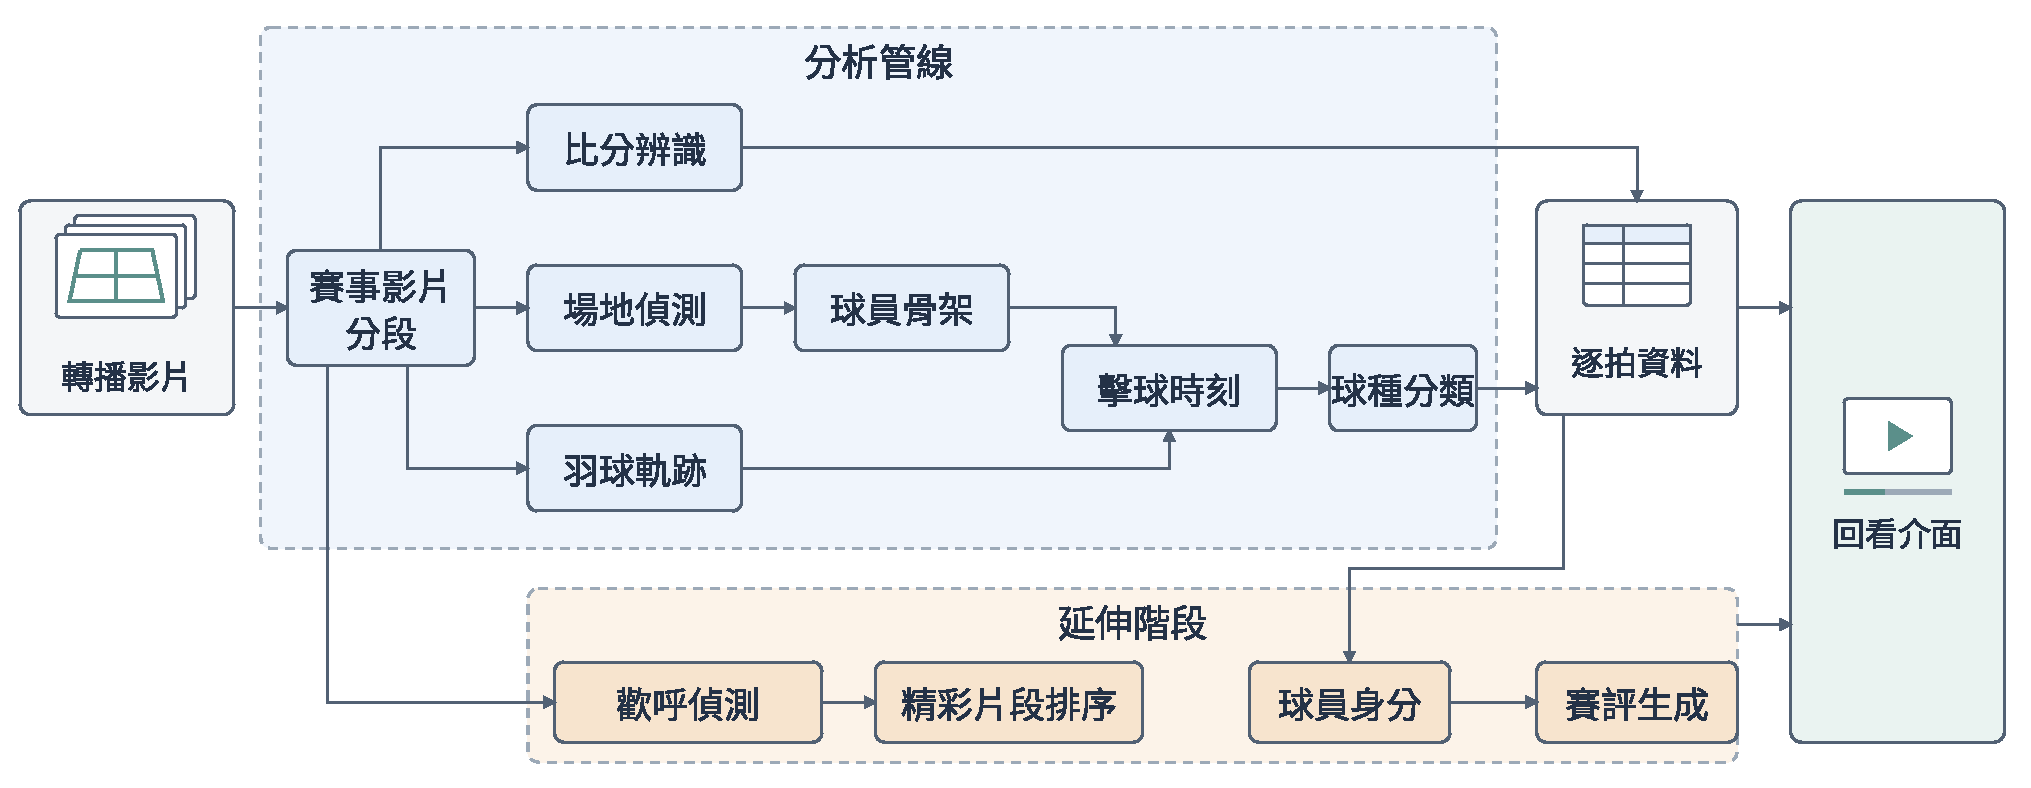
\includegraphics[scale=\flowscale]{system-overview.pdf}
  \caption[系統概觀]{系統概觀。分析管線將轉播影片轉為逐拍資料，延伸階段與回看介面建立在其產出之上。}
  \label{fig:system-overview}
\end{figure}

系統由三部分組成（\figref{fig:system-overview}）：把轉播影片轉成逐拍資料的分析管線、建立在管線產出之上的延伸階段，以及對照影片檢視結果的回看介面。分析管線依序處理以下步驟：

\begin{enumerate}
  \item \textbf{界定分析範圍。}轉播影片中夾雜重播、特寫等畫面，賽事影片分段先找出主機位的比賽片段，後續所有分析都只在這些片段內進行。比分辨識再讀出每個片段計分板上的比分，讓片段能對應回比賽中的比分。
  \item \textbf{定位球場、球員與羽球。}場地偵測定位球場範圍，建立畫面與球場平面之間的對應。球員骨架追蹤據此從裁判、線審與觀眾之中挑出場上的兩名球員。球體追蹤則逐影格定位羽球，重建羽球軌跡。這三項是後續擊球分析共同需要的輸入。
  \item \textbf{找出每一拍並分類。}擊球時刻偵測結合羽球軌跡與球員骨架，找出每一次擊球的影格。球種分類再依每一拍前後的骨架、軌跡與球場位置，判斷球種。
\end{enumerate}

管線之外另有四個延伸階段。球員身分對應依比分與發球者，把上下方對應到具體選手。賽評生成再以逐拍結果與球員身分為事實依據，由大型語言模型撰寫賽評，並逐句檢查是否有資料支持。歡呼偵測量測每個片段結束前後的觀眾歡呼，精彩片段排序據此為片段排出精彩程度。

回看介面（\figref{fig:review-workspace}）除了對照影片檢視所有結果，也能直接發起分析任務。各模組的設計與實作見\chapref{ch:system-design}。

\begin{figure}[H]
  \centering
  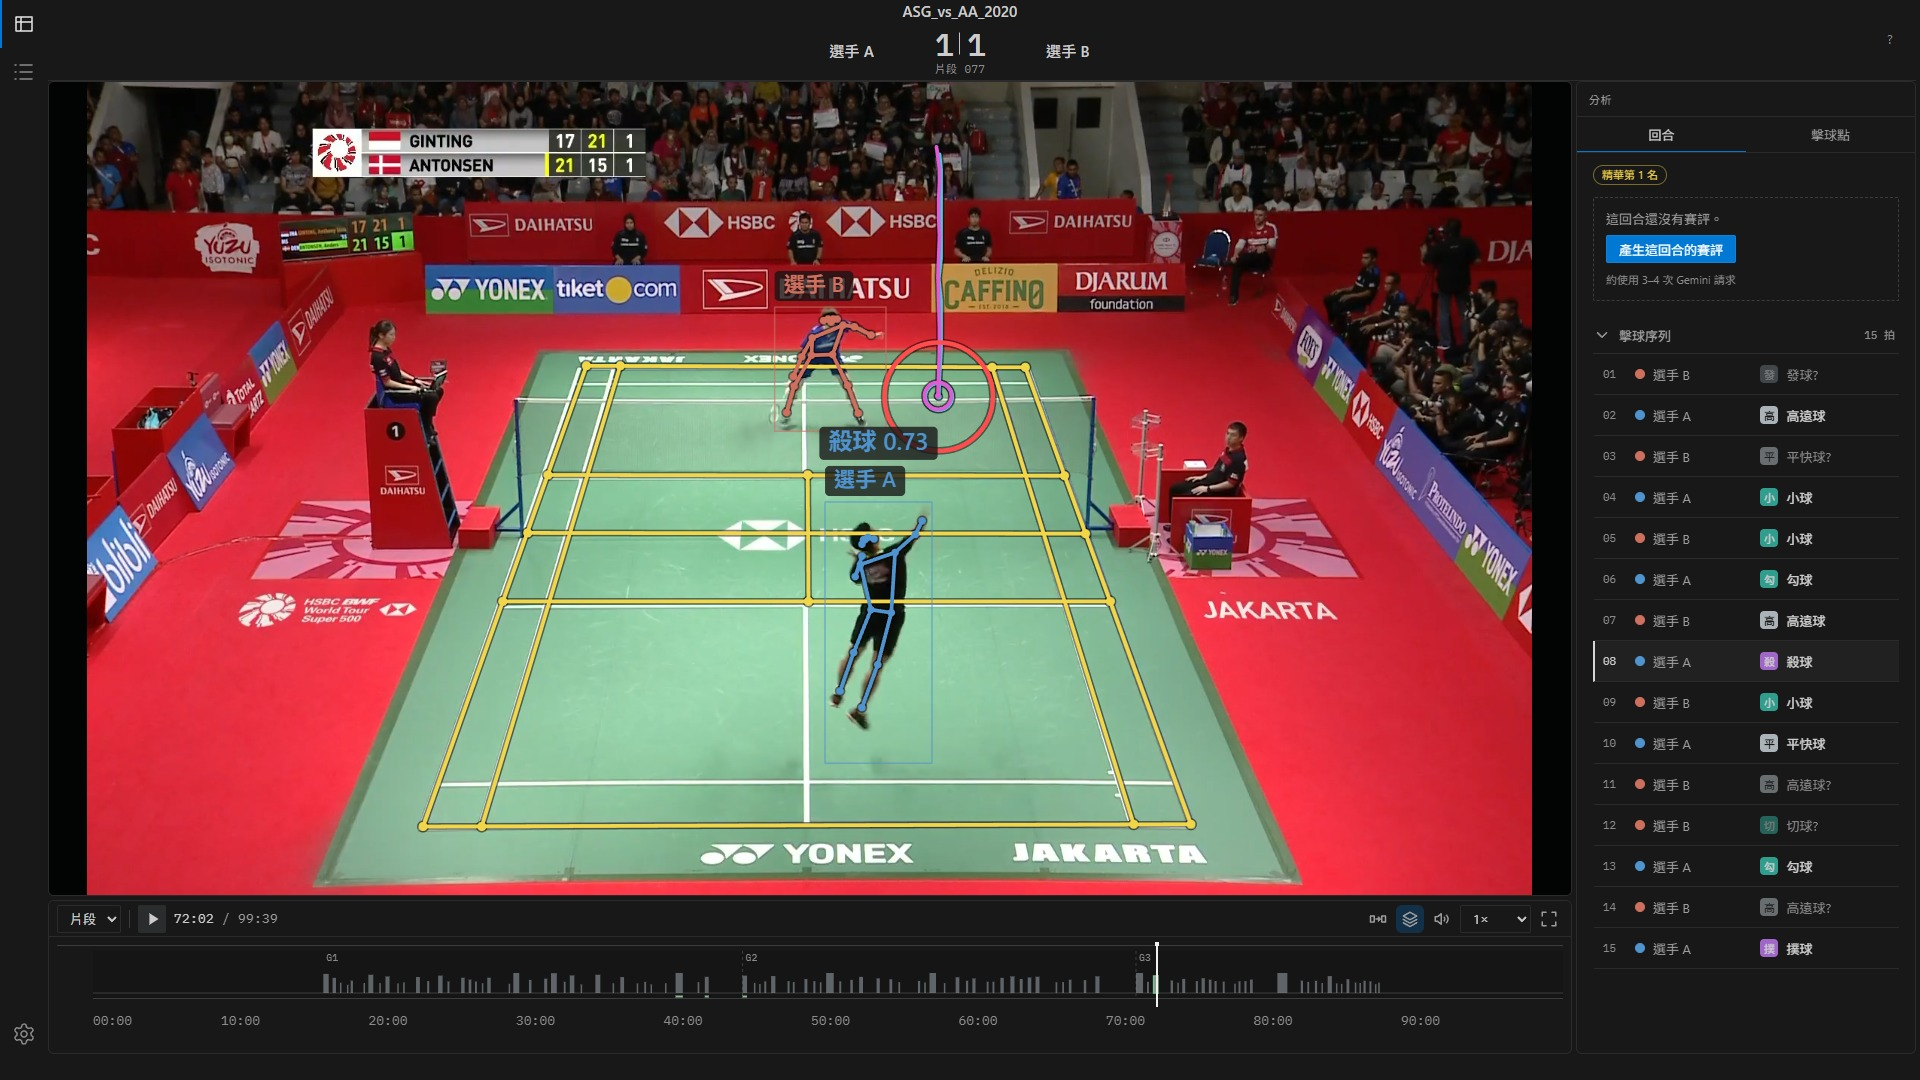
\includegraphics[width=\linewidth]{ui/review_workspace_clean.jpg}
  \caption{回看介面}
  \label{fig:review-workspace}
\end{figure}

\section{主要貢獻}
\label{sec:contributions}

上述各模組多有既有方法可以參考，但如\secref{sec:motivation}所述，這些方法預設輸入已經整理好，比賽片段起訖、球場範圍與擊球時刻都由人工提供。與既有的整合系統及開源專案相比，本系統的主要貢獻有以下四點。

\begin{enumerate}
  \item \textbf{把既有方法所依賴的上游自動化。}比賽片段起訖、球場範圍與擊球時刻在資料集中原由人工提供，本系統分別以影格差異訊號分段、由內部線條反推範圍的場地偵測，以及融合軌跡、骨架與球種證據的擊球時刻偵測取得，不需針對每支影片人工標記或調整參數。TrackNetV3~\cite{tracknetv3}、BST~\cite{bst} 等既有模型因此能直接在未經處理的轉播影片上運作。
  \item \textbf{模組化、可局部重跑的管線。}各模組仍在持續改進，因此每個階段都能單獨替換與重跑。階段之間只透過統一的資料契約溝通，執行器以上游產物的內容雜湊判斷結果是否過期，中間結果以片段為單位快取。調整其中一個模組時，只需重算受影響的部分。
  \item \textbf{公開、可重現的評估。}實驗使用 16 支 YouTube 公開的單打完整轉播，以影片為單位切分為開發集與測試集。我們公開每支影片的雜湊與影格指紋，讓他人能確認自己下載的影片與我們標記時所用的一致。真值、評分程式與逐場結果也一併公開。
  \item \textbf{應用示範：以比賽事實約束生成式 AI 的賽評。}為展示逐拍資料的下游價值，我們在管線之上建立賽評生成，重點在於避免大型語言模型的幻覺。每一拍的時刻、擊球者與球種都取自管線結果，模型只負責措辭，產生的賽評再經審查比對分析結果，沒有資料支持的句子改以只陳述事實的模板句取代。
\end{enumerate}

\section{效能評估結果}
\label{sec:results-summary}

\tabref{tab:results-summary}列出各模組的代表指標，完整實驗與失敗案例分析見\chapref{ch:experiments}。

\begin{table}[H]
  \centering
  \small
  \caption{各模組的代表指標}
  \label{tab:results-summary}
  \begin{tabularx}{\linewidth}{|l|L|l|L|}
    \hline
    模組 & 評估資料 & 主要指標 & 其他指標 \\ \hline
    賽事影片分段 & 測試集 9 場、670 個片段 & F1 98.66\%（IoU $\geq$ 0.9） & 邊界誤差中位數 0 影格 \\ \hline
    場地偵測 & 測試集 9 場、36 個外角 & 命中率 72.22\% & 誤差中位數 2.79 像素，6 場四角全中 \\ \hline
    擊球時刻偵測 & 測試集 8 場、6,990 拍 & F1 93.14\%（$\pm$5 影格） & Precision 95.49\%、Recall 90.90\% \\ \hline
    歡呼偵測 & 開發用 4 場逐場留一，外部 1 場 & Macro F1 82.70\% & ROC-AUC 0.96 \\ \hline
    處理時間 & 5 場、片長 332 分（片段 98 分） & 片段總長的 2.71 倍 & 扣除 API 等待後 1.96 倍（RTX 3060 Ti） \\ \hline
  \end{tabularx}
\end{table}

分段與擊球時刻偵測的 F1 皆超過 93\%，已可直接供下游使用。最弱的一環是場地偵測，未命中的角幾乎都源於底線旁的廣告字樣，且系統目前無法自行察覺。16 支影片中有 15 支來自 BWF 官方轉播，跨轉播單位的泛化尚未驗證。歡呼偵測僅以 4 場開發比賽與 1 場外部驗證評估。處理時間未計入音訊、身分對應與賽評等延伸階段。

\section{報告組織}
\label{sec:organization}

本報告其餘章節安排如下。\chapref{ch:related-work}回顧既有的整合系統與各子任務的方法，歸納研究缺口與本系統的定位。\chapref{ch:system-design}先說明管線架構與階段間的約定，再依處理順序介紹各模組的設計，包括影片前處理、場景與人體理解、球體分析、音訊與精彩度分析、賽事理解，最後介紹使用者介面。\chapref{ch:experiments}說明資料集與重現方式，報告各模組與端到端的實驗結果。\chapref{ch:conclusion}討論系統的優點與限制，並總結本專題與未來工作。附錄說明開發過程中生成式 AI 的使用方式。
